\documentclass[11pt]{article}
\usepackage{geometry}                
\geometry{letterpaper} 
\usepackage{graphicx}
\usepackage{amssymb}
\usepackage{epstopdf}
\usepackage{amsmath}
\usepackage[round]{natbib}
\DeclareGraphicsRule{.tif}{png}{.png}{`convert #1 `dirname #1`/`basename #1 .tif`.png}

\title{Casimir Force in Microgravity Experiment}
\author{Noah Kurinsky}
%\date{}                                  

\begin{document}
\maketitle

\section{Expanded Proximity Force Approximation}
Most of this section taken from \citet{Dexp}

Normal energy of Casimir Effect:
$$
E_{pp}(z)=-\frac{\pi^2}{1440z^3}
$$

For $R>>a$:
$$
E_{C}\approx E_{PFA}=\int_{\Sigma}E_{pp}(z)d\sigma
$$

We don't expect this to hold much past this condition, but can use the derivative expansion to first order to obtain a slightly more accurate term. The formula for the derivative expansion in terms of some surface separation $z=\psi(\mathbf{x}_\parallel)$ is
$$
E_{DE}=-\frac{\pi^2}{1440}\int\frac{1}{\psi^3}\left(1+\frac{2}{3}(\partial_\alpha \psi)^2\right)d\mathbf{x}_\parallel
$$
and if we add in the correction factor $\eta_E(z)$ (see next section), we get
$$
E_{DE}=-\frac{\pi^2}{1440}\int\frac{\eta_E(\psi)}{\psi^3}\left(1+\frac{2}{3}(\partial_\alpha \psi)^2\right)d\mathbf{x}_\parallel
$$
which, given the complexity of $\eta_E$, is best evaluated numerically. We can parameterize the surface of a sphere as
$$
\psi_0(r)=R\left(1-\sqrt{1-\frac{r^2}{R^2}}\right)
$$
where the surface separation would be $\psi=a+\psi_0(r)$ and $a$ the minimal separation between sphere and plane. Given that the derivative with respect to $\theta$ is 0, the integral simplifies to
$$
E_{DE}=-\frac{2\pi^3}{1440}\int\frac{\eta_E(\psi)}{\psi^3}\left(1+\frac{2}{3}(\partial_r \psi)^2\right)dr
$$
and we can write, as well, 
$$
(\partial_r\psi)^2=R^2\left[-\frac{1}{2}\left(1-\frac{r^2}{R^2}\right)^{-1/2}\left(\frac{-2r}{R^2}\right)\right]^2=\frac{r^2}{R^2(1-\frac{r^2}{R^2})}=\frac{r^2}{R^2-r^2}=\left(\frac{R^2}{r^2}-1\right)^{-1}
$$
we can see that the derivative is undefined if we integrate to $R$, so as long as we integrate to $r_{limit}<R$ we should have a convergent integral; this shouldn't affect the accuracy given the $r^{-3}$ dependence. The effect of the derivative expansion correction in a perfectly conducting system can be seen below.

\begin{figure}[h]
\centering
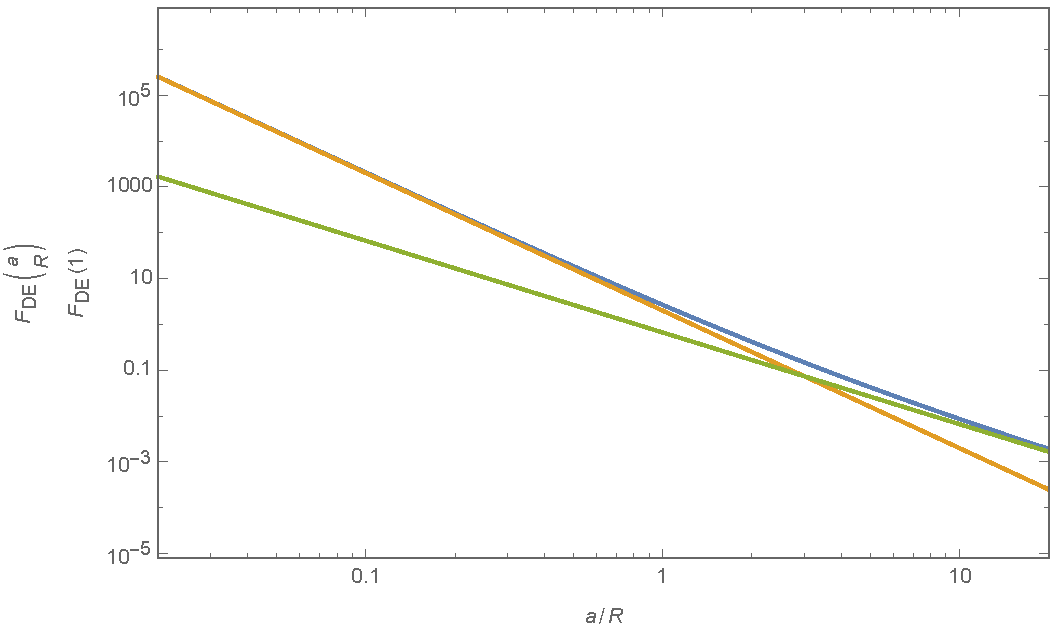
\includegraphics[width=5in]{PFAExpansion}
\caption{Illustration of the effect of the first order correction on the PFA; blue line shows expansion, orange line is PFA, green line is first order correction.}\label{fig:expansion}
\end{figure}

\citet{Bulgac} calculate the force between plane and sphere exactly, and compare to PFA. \citet{Durand} explore various temperature and geometry effects as a function of radius and separation. 

\subsection{Dielectric Correction}
\citet{BeyondPFA,Lambrecht}: dielectric effects, non-perfect conductivity. The following mostly from \citet{Lambrecht}

The dielectric constant is large at frequencies smaller than the plasma frequency $\omega_p$, so corrections are more relevant at separations smaller than the plasma wavelength
$$
\lambda_p=\frac{2\pi c}{\omega_p}
$$
where
$$
\omega_p^2=\frac{Nq^2}{\epsilon_0m^*}=\frac{ZN_aq^2}{\epsilon_0m^*}=\frac{\rho q^2}{\epsilon_0m^*m_z}
$$
and in turn, $N$ is the number of conduction electrons per unit volume, $Z$ is the number of free electrons per atom (taken to just be $Z=1$), $N_a$ is the atomic number density, $q$ is the electron charge, and $m^*$ is effective electron mass, also taken to be 1 for Au though not necessarily for $\mathrm{SiO^2}$. We in turn calculate $N_a$ as the density $\rho$ divided by the atomic mass $m_Z$ for the species.

Thermal corrections relevant at distances larger than 
$$
\lambda_T=\frac{\hbar c}{k_B T}
$$
The reduction factor for the Casimir energy is given by
\begin{equation}
\eta_E=-\frac{180L^3}{c\pi^4}\int^{\infty}_{0}\kappa d\kappa\int^{c\kappa}_0\sum_{p=\parallel,\perp}\log{\left(1-r_{p,1}(i\omega,i\kappa)r_{p,2}(i\omega,i\kappa)e^{-2\kappa L}\right)}d\omega
\end{equation}
where $r_{p,i}(i\omega,i\kappa)$ is the reflection amplitude of surface $i$ for polarization $p$, where $i\omega$ is the imaginary frequency and $i\kappa$ is the imaginary wave vector along the longitudinal direction of the cavity, or the normal to the plane. The reflection coefficients for thick slabs are given by
\begin{align}
r_{\perp}&=-\frac{\sqrt{\omega^2(\epsilon(i\omega)-1)+c^2\kappa}-c\kappa}{\sqrt{\omega^2(\epsilon(i\omega)-1)+c^2\kappa}+c\kappa} \\
r_{\parallel}&=\frac{\sqrt{\omega^2(\epsilon(i\omega)-1)+c^2\kappa}-c\kappa\epsilon(i\omega)}{\sqrt{\omega^2(\epsilon(i\omega)-1)+c^2\kappa}+c\kappa\epsilon(i\omega)}
\end{align}

\citet{Lambrecht} suggest numerical integration over the range $10^{-4}$ to $10^{3}$ eV for distances 0.1 to 10 $\mu$m

\subsection{Expected accuracy}
We are limited by the validity of the proximity force approximation, which assumes the (roughly) Casimir forces are additive, which is known not to be the case, and assumes the sphere and plane are close enough such that the plane appears infinite and the curvature is relatively small. We include the first order correction to the PFA, which may not extend validity very far and still assumes the plane is long enough to be effectively infinite.

\section{Numerical Computation}

\pagebreak
\appendix
\section{Scuff-EM}
\section{Casimir Force Code}

\bibliographystyle{plainnat}
\bibliography{Casimir}

\end{document}  